\section{Overview}\label{sec:Overview}

A critical precursor to robot path planning is the ability to determine a robot's pose relative to a known environment.
The problem of estimating a robot's pose relative to a known map from proprioceptive and exteroceptive measurements is referred to as localization \cite{thrun2005probabilistic}.
Without a reliable estimate of a robot's state with respect to the world, a robot cannot safely interact with its surroundings.
This paper presents a study comparing algorithms for performing localization of a differential drive mobile manipulator equipped with a two-dimensional (2-D) Light Detection and Ranging (LiDAR) sensor and wheel odometry.
Each algorithm approximates a probability distribution for the pose, called the \textit{belief}.

To facilitate the development of the algorithms, this study utilizes the Robot Operating System 2 (ROS2) \cite{macenski2022ros2}.
ROS2 is a middleware framework that is built on top of the Data Distribution Service (DDS) protocol \cite{pardo2003omg} to support distributed architectures.
Within the ecosystem, independent processes are referred to as ``nodes.''
Nodes communicate with one another by publishing and subscribing to shared message queues known as ``topics.''
The distributed architecture enables asynchronous processing of sensor data and commands.

Additionally, this study utilizes the Gazebo simulation environment, which provides a high-fidelity physics engine and sensor simulation plugins.
The experiments are conducted in a simulated factory world populated with obstacles and goal points for navigation.
Figure \ref{fig:gazebo_sim_2d} illustrates the factory layout, goal points, and the initial position of the robot in 2-D.
Figure \ref{fig:gazebo_sim_3d} provides a screenshot of the factory at runtime in three dimensions (3-D).

\begin{figure}[!htbp]
    \centering
    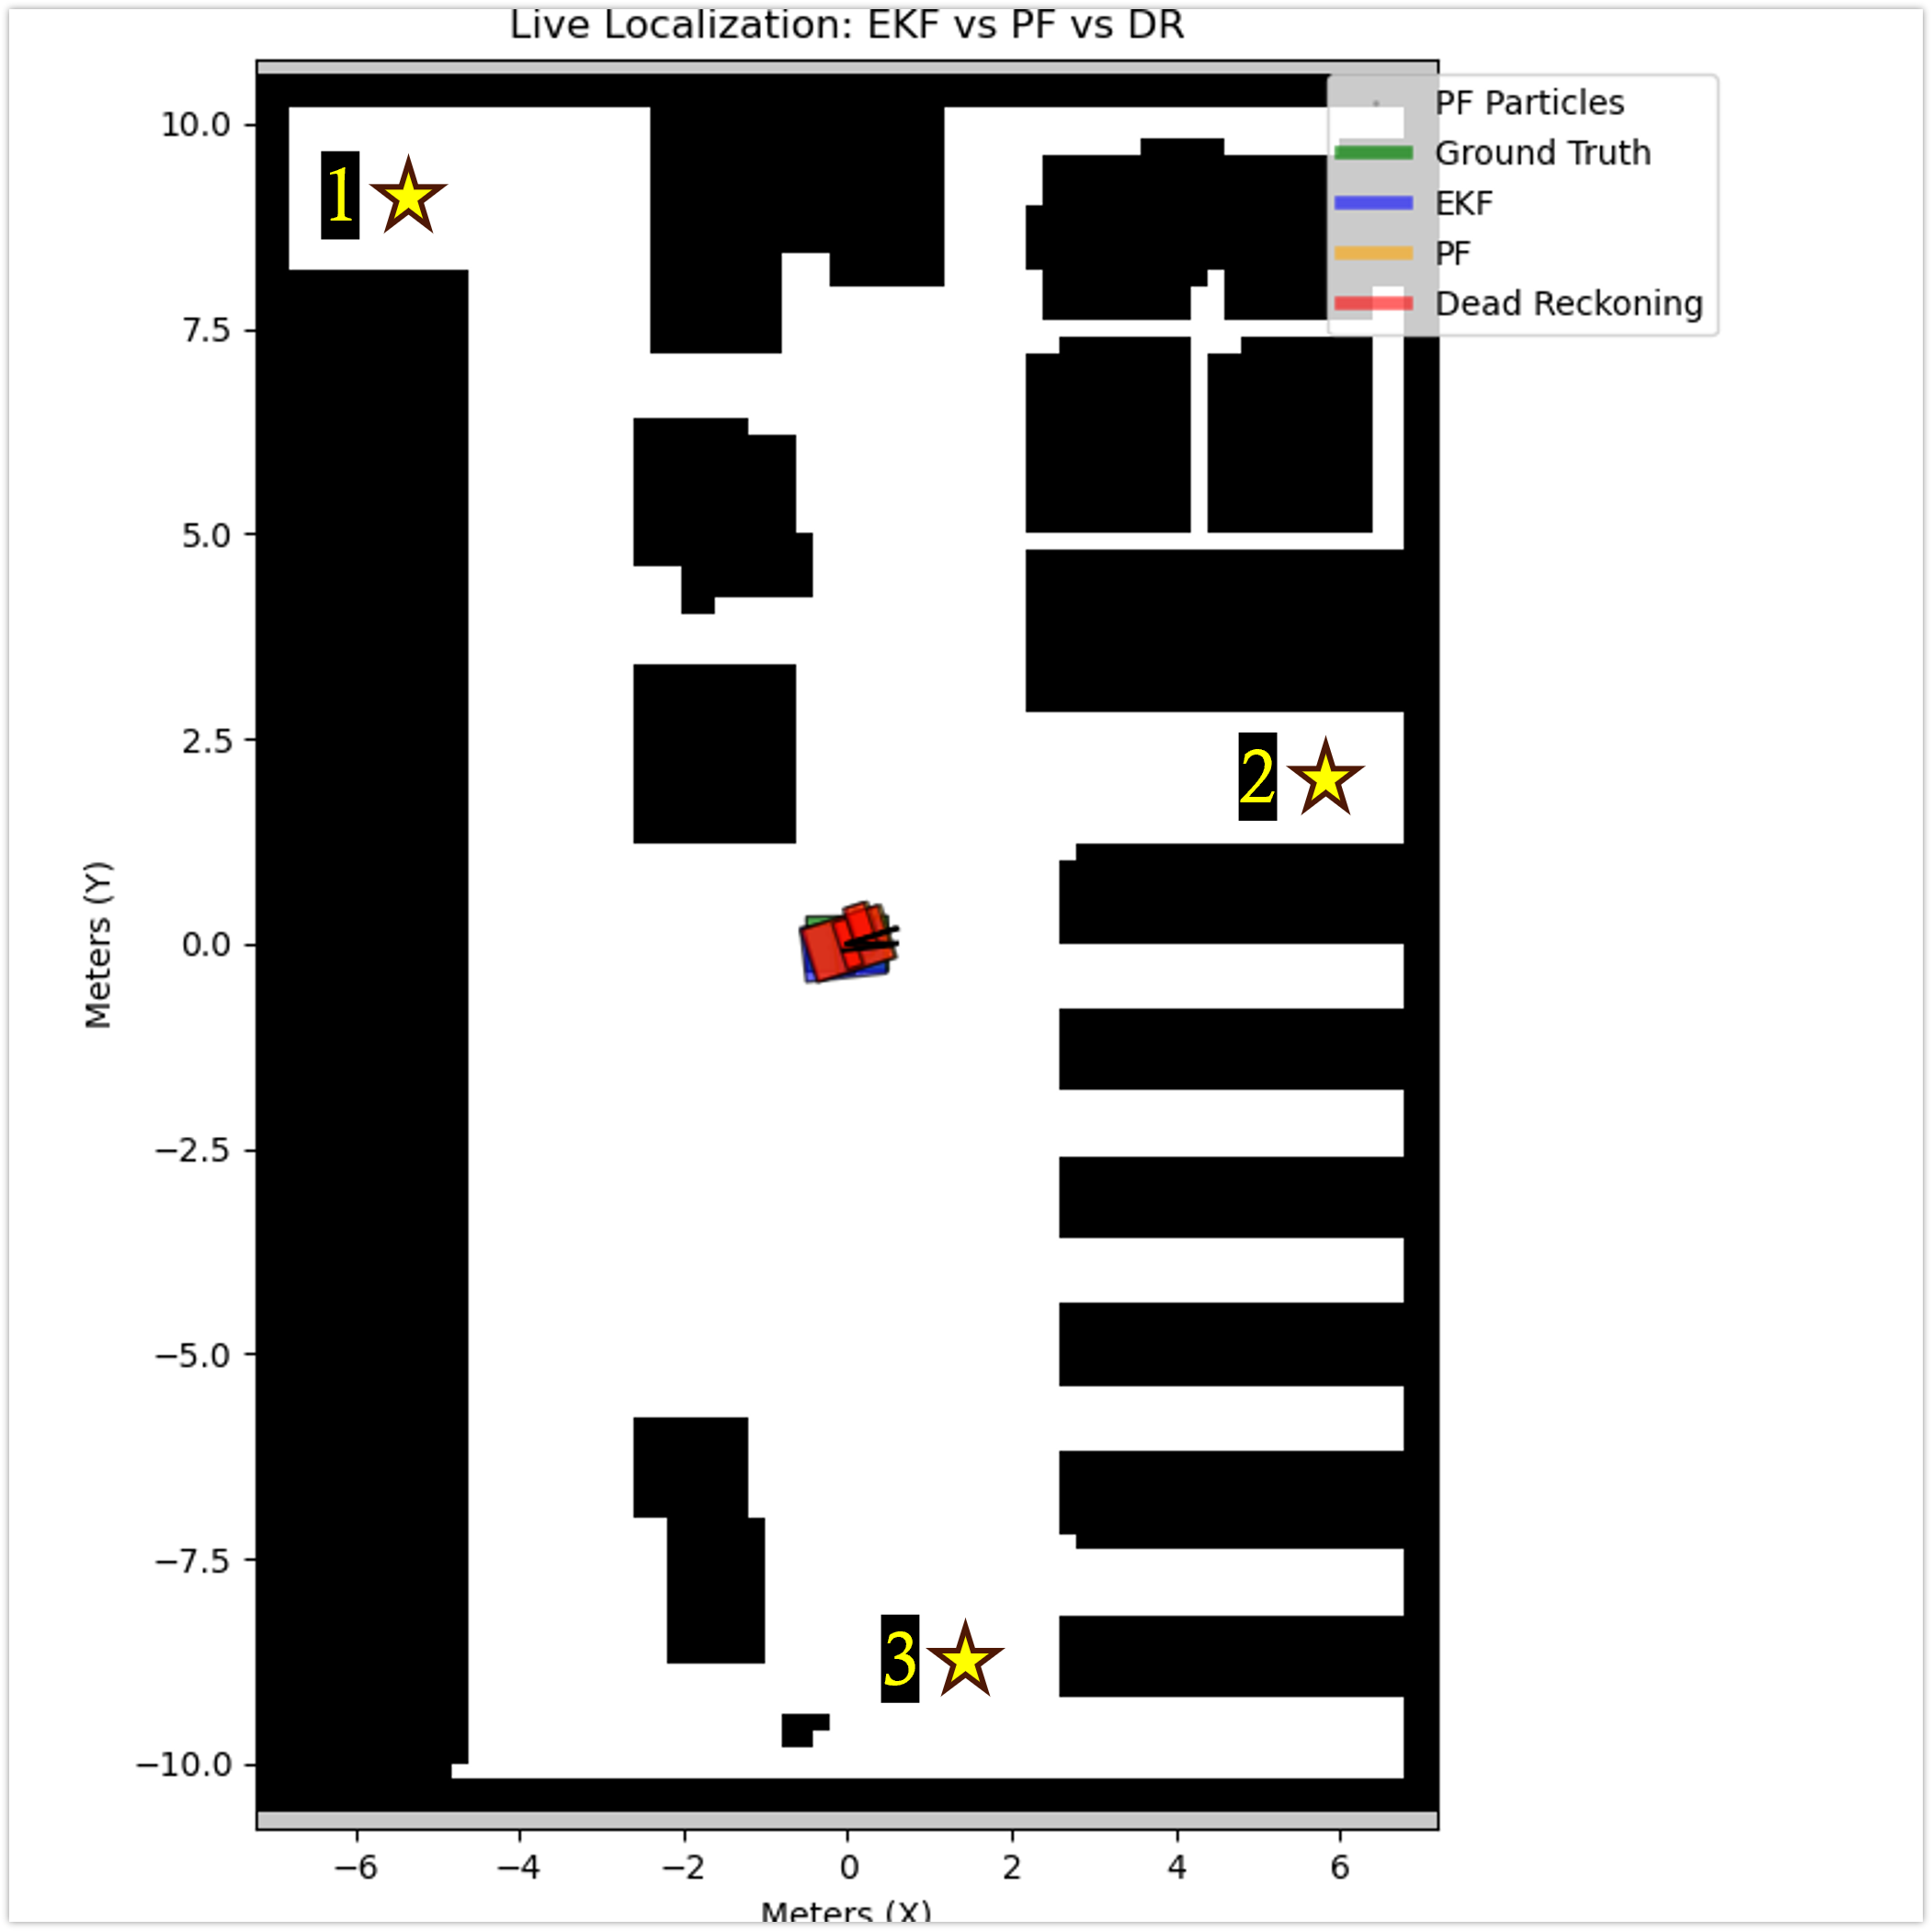
\includegraphics[width=0.6\textwidth]{figures/Devol_Localization_Viz_labeled.png}
    \caption{2-D Rendering of the factory floor, obstacles, and designated goal points.}
    \label{fig:gazebo_sim_2d}
\end{figure}

\newpage

\begin{figure}[!htbp]
    \centering
    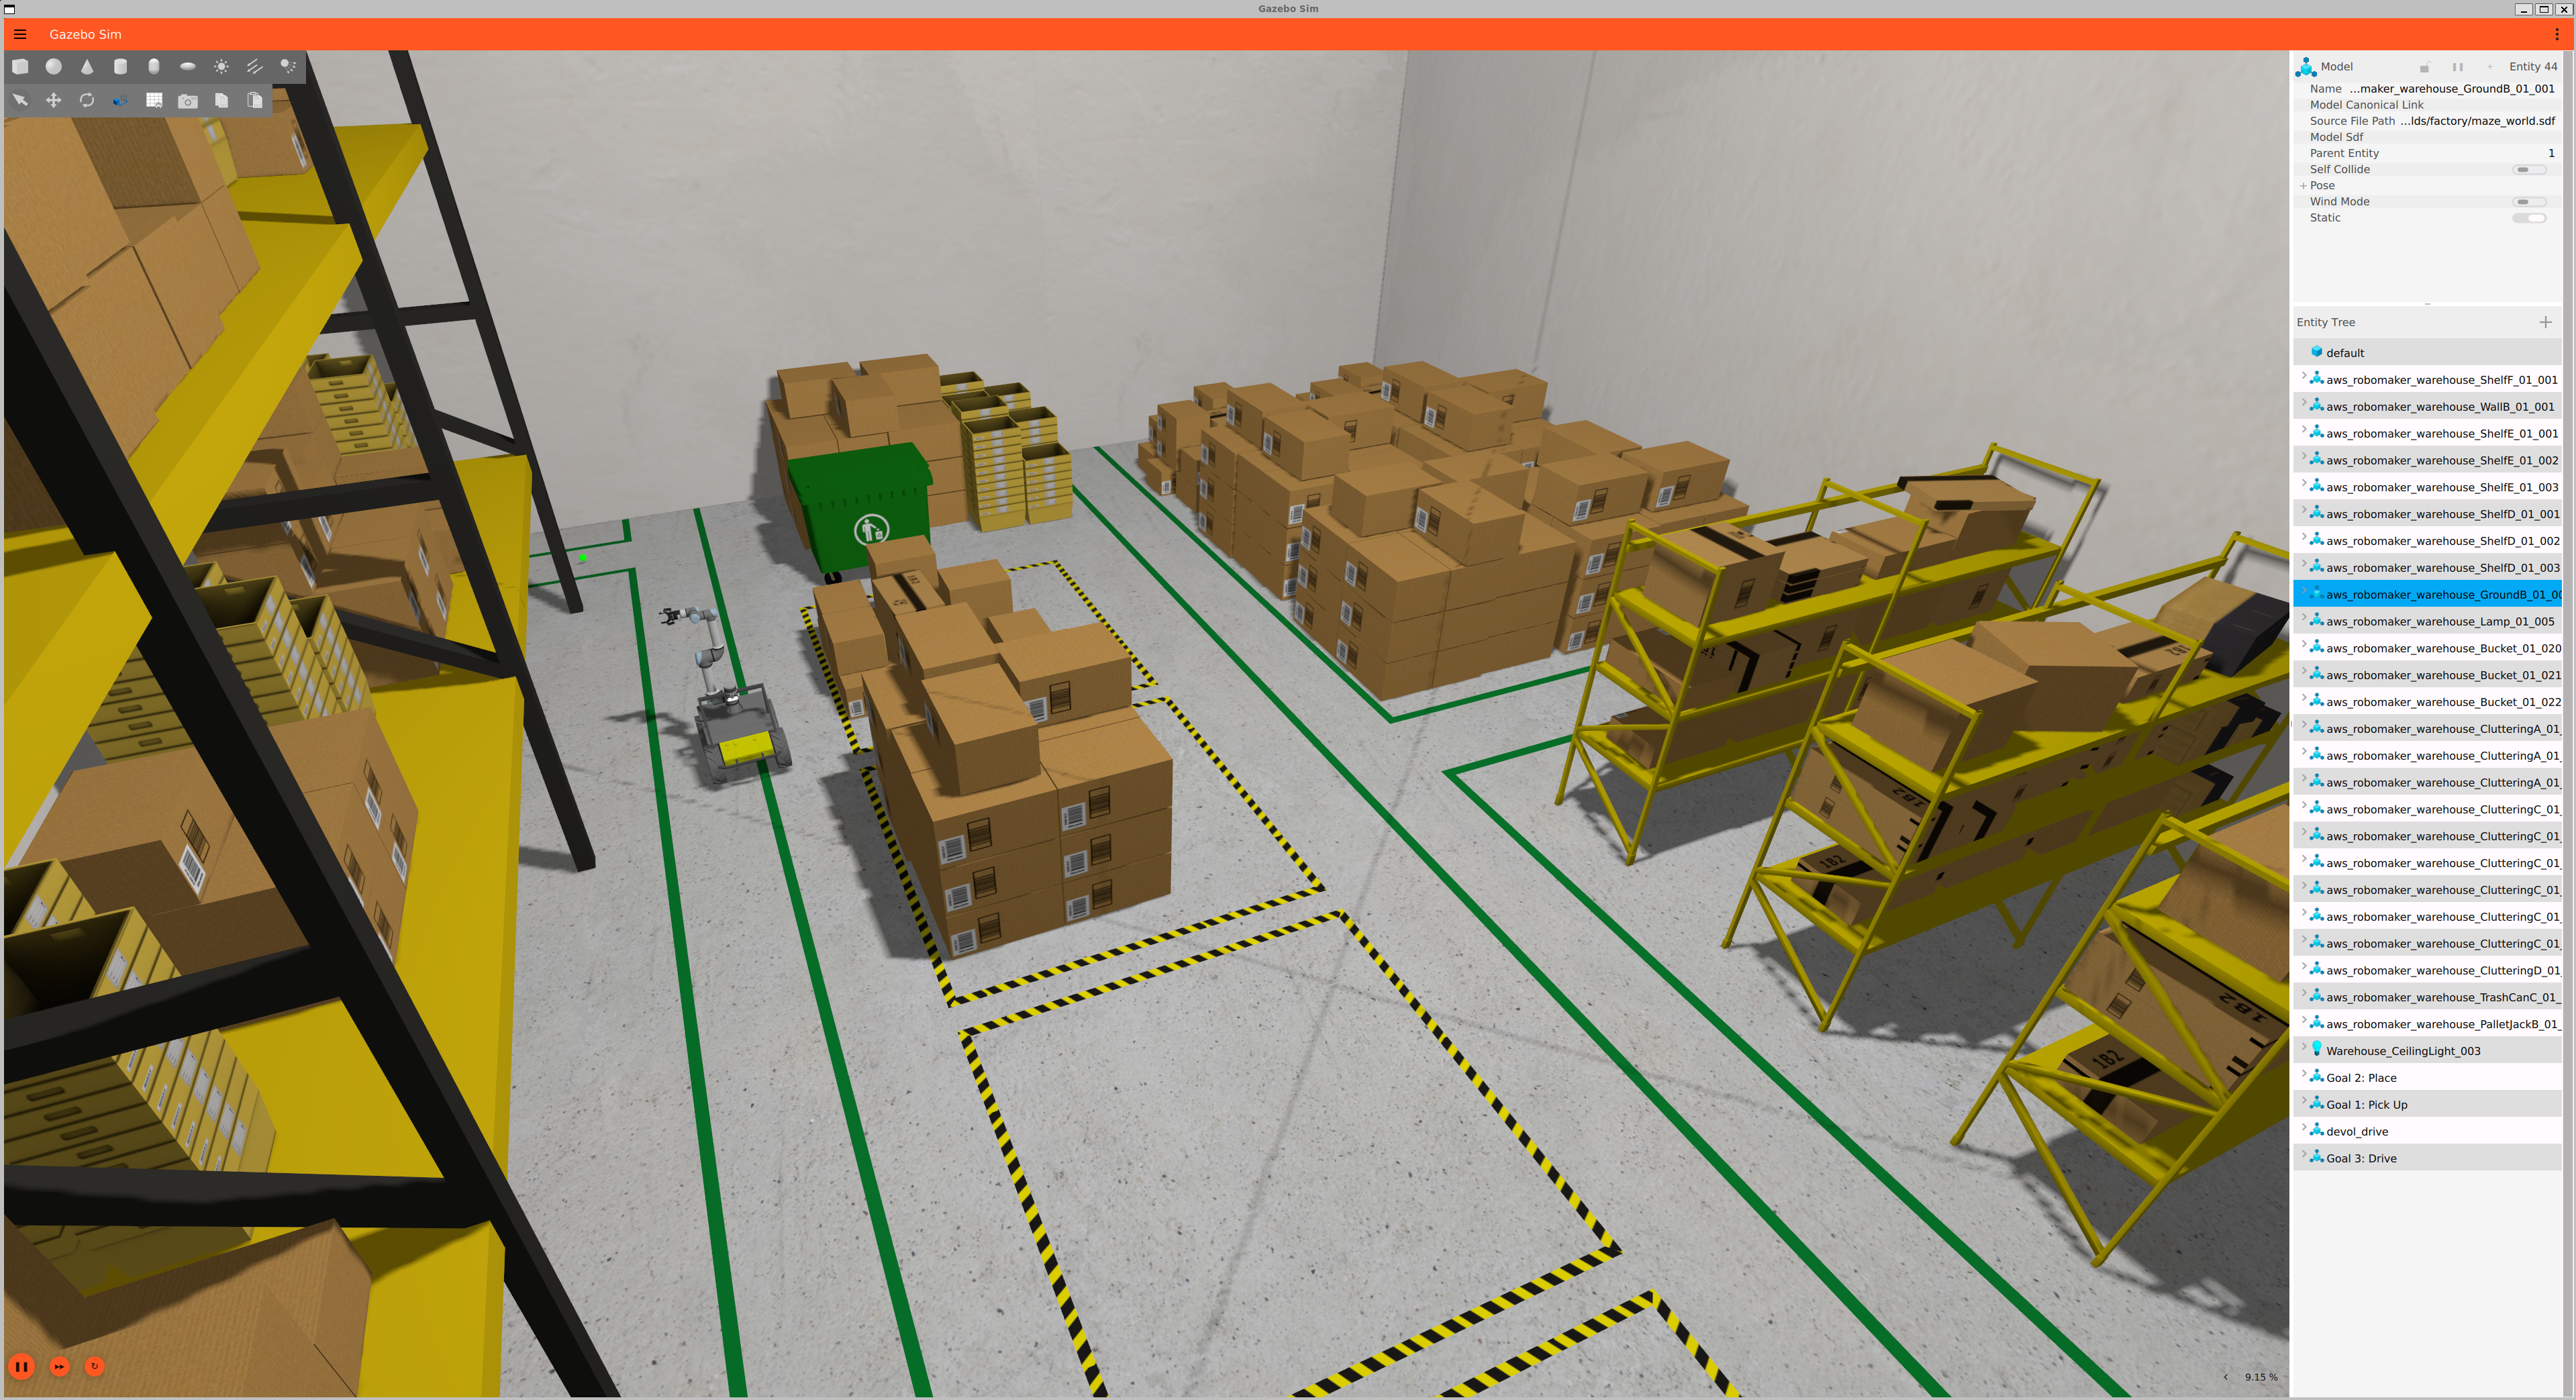
\includegraphics[width=\textwidth]{figures/gazebo_screenshot.png}
    \caption{Gazebo factory 3-D simulation.}
    \label{fig:gazebo_sim_3d}
\end{figure}

The primary objective of this study is to evaluate and compare the performance of different localization algorithms when deployed on a mobile manipulator in a factory setting. 
Specifically, this work investigates the trade-offs between Dead Reckoning, Extended Kalman Filter, and Particle Filter approaches. 
By analyzing localization accuracy, computational efficiency, robustness to sensor noise, and kidnapping recovery, this study aims to provide practical insights into selecting the appropriate state estimation strategy for autonomous mobile manipulation.